\documentclass[oneside,final,14pt]{extreport}
\usepackage[utf8]{inputenc}
\usepackage[russian]{babel}
\usepackage{vmargin} \setpapersize{A4}
\setmarginsrb{2cm}{2cm}{2cm}{2cm}{0pt}{0mm}{0pt}{13mm}
\usepackage{indentfirst}
\usepackage{graphicx}
\usepackage{amsmath}
\usepackage{amsfonts}
\setcounter{secnumdepth}{0}

\begin{document}

\begin{titlepage}
\begin{center}
    {\bfseries Алгоритмы и анализ сложности.} \\
    \vspace{\fill}
    Анализ алгоритма Тарьяна для поиска \\ компонент сильной связности 
    в орграфе.
\end{center}
\vspace{\fill}
    \begin{flushright}
        Волокитин Егор \\ 20.Б12 - ПУ
    \end{flushright}
\end{titlepage}

\newpage

\tableofcontents

\newpage
\section{Основные определения и краткое описание алгоритма.}

\noindent
{\itshape \underline{def.}} Орграф - это ориентированный граф, т.е. граф,
рёбрам которого присвоено направление.

\noindent
{\itshape \underline{def.}} Сильно связный орграф - ориентированный граф,
в котором все его вершины взаимно достижимы, т.е. между двумя любыми
вершинами $a$ и $b$ существует ориентированный путь из $a$ в $b$ и из $b$ в
$a$.

\noindent
{\itshape \underline{def.}} Компоненты сильной связности орграфа - это
максимальные по включению сильно связные подграфы орграфа.

\bigskip
\noindent
Алгоритм Тарьяна для поиска компонент сильной связности в орграфе был
открыт Робертом Андре Тарьяном в 1972 году. Этот алгоритм на вход принимает
ориентированный граф, представленный в виде двух множеств: множества вершин
и множества рёбер. Во время работы мы получаем множество вершин, которые 
входят в одну и ту же компоненту сильной связности, записываем их,
и продолжаем искать другие компоненты, пока не пройдём все вершины.
Алгоритм работает за линейное время.


\bigskip
\noindent
Данный алгоритм очень похож на алгоритм обхода графа в глубину (в каждую 
вершину мы заходим только один раз), в котором
при посещении веришины, и при выходе из неё делались бы дополнительные 
дейстия.

\bigskip
\noindent
Вершину можно представить как структуру данных из трёх полей: \\
\indent $index$ - сколько вершин мы обработали до этой, т.е. какой по 
счёту обрабатываем данную вершину \\
\indent $lowlink$ - нименьший $index$ вершины, которая находится
в одной компоненте свзязности с данной вершиной \\
\indent $on\_stack$ - находится ли данная вершина в стеке, нужно для
проверки есть ли вершина в стеке за константное время.

\bigskip
\noindent
Мы последовательно начинаем перебирать вершины, и если у неё $index$ не 
равен $null$, то пропускаем её, иначе начинаем её обрабатывать.\\
Во-первых присвоим её полям $index$ и $lowlink$ значение $global\_index$, 
которое говорит, какой по счёту мы обрабатываем данную вершину.\\
Во-вторых положим эту вершину на стек, и изменим значение поля 
$on\_stack$.\\
Далее начинаем поиск в глубину, а именно, смотрим в какие вершины можно 
перейти из текущей вершины. \\
1) Мы можем перейти в вершину, в которой никогда не были. \\
Тогда начинаем рекурсивно обрабатывать эту вершину, а после обработки
смотрим на значение её $lowlink$. Если у этой вершины значение больше, 
чем у текущей вершины, значит они в разных компонентах свзяности, иначе мы 
записываем в значение текущей вершины, значение $lowlink$ вершины, в
которую мы смотрели.\\
2) Мы можем перейти в вершину, которая уже на стеке. \\
Если вершина уже на стеке, значи мы её когда-то проходили, значит опять же
сравниваем значения $lowlink$ и текущей вершине присваиваем минимальное. \\
Итак, мы прошли все возомжные пути из данной вершины, и теперь смотрим,
если значение $index$ совпало с $lowlink$, то значи мы находимся в корне
компоненты сильной связности, и начинаем снимать и запоминать значения со
стека, пока не дойдём до текущей корневой вершины. Эти значения и будут
компонентой связности.

\newpage
\section{Математический анализ алгоритма.}

\noindent
Для каждой вершины $v$ из множества вершин $V$ функция обработки будет
вызываться только один раз, либо при общем обходе вершин, либо уже
рекурсивно из функции обработчика, 
но алгоритм никогда не запустит обработку для вершины, которую
уже обработали.\\ 
Внутри функции обработки есть цикл, который перебирает все
рёбра, которые выходят из данной вершины. Но если ребро выходит из одной
вершины, то значит оно не выходит не из какой другой, значит при вызове
обработчика для вершины $a$ мы возьмём тольк часть рёбер из множеста рёбер
$|E|$,
причём эта часть рёбер не будет пересекаться ни с какими другими рёбрами,
которые будем рассматривать для других вершин. Значит каждое ребро мы
рассматриваем только один раз. \\
Также внутри функции обработчика все действия выполняются за константное
время, даже проверка есть ли вершина в стеке, благодаря структуре вершин. \\
Также, мы кладём на стек сумарно столько вершин, сколько у нас есть в 
графе. \\
Значит мы делаем $k_1 * |V| + k_2 * |E| + k_3$ действий, а значит
затрачиваем линейное время на выполнение: $$O(|V| + |E|)$$

\bigskip
\noindent
Вообще, расходы на дополнительную память будут различными, в зависимости от
того, как именно реализуется алгоритм.\\
Сразу видно, что большая часть дополнительной памяти будет выделена под
стек, на котором будут хранится вершины. Можно сэкономить место, и хранить
не всю вершину, а лишь ссылку на неё. В худшем случае на стеке будут 
хранится сразу все вершины, если у нас весь граф одна большая компонента
сильной связности.\\
Потом дополнительные расходы вызовёт то, что мы делаем саму структуру
вершин, в которой хранятся два вида индексов, информация о нахождении в
стеке, информация о статусе обработки данной вершины. \\
Все расходы на дополнительную память связаны с вершинами, а точнее с их
количеством, причём это можно описать как $x * |V|$, где $x$ - это
количество байт на хранение структуры вершин, плюс $y * |V|$, $y$ - это
количество байт на ссылку в стеке, причём это при худшем случае. \\
Расходы на хранение рёбер не беру в расчёт, так как это не дополнительные
расходы, а изначально предоставленные данные.
По итогу на дополнительную память будет потрачено: $$O(|V|)$$

\newpage
\section{Описание генератора входных данных.}

\noindent
Посмотреть на генератор данных можно в репозитории с проектом
(см. список литературы -> generator.cpp) \\
Основной принцип его работы такой: \\
1) Задаётся количество вершин в графе. \\
2) Для каждой вершины запускается цикл $for$, где счётчиком являются другие
вершины. \\
3) С заданной вероятностью между выбранной вершиной, и вершиной-счётчиком
создаётся ребро, или не создаётся.\\
У генератора есть два основных параметра - количество вершин и вероятность
появления ребра между двумя вершинами(не обязательно двумя разными)
Также можно смотреть на то, сколько рёбер создалось.\\
Генератор был сделан таким образом, потому что на время работы алгоритма
влияют количество вершин и рёбер, и по этим значениям удобнее всего
анализировать зависимости.


\newpage
\section{Описание реализации алгоритма.}

\noindent
Реализацию алгоритма с подробными комментариями можно посмотреть в 
репозитории (см. список литературы -> tarjan.cpp) \\
Если говорить о самой программе, то она устроена следующим образом:\\
1) Задаются основные параметры генератор (количество вершин и вероятность
появления ребра между двумя вершинами)\\
2) Генерируется массив рёбер.\\
3) Потом на одном и том же массиве рёбер 1000 раз запускается алгоритм,
подсчитывается суммарное время выполнения алгоритма 1000 раз, потом делится
на 1000, и таким образом получается среднее время выполнения алгоритма.\\
4) На экран выводится результат среднего времени, количества рёбер
и количество вершин.\\
5) Также предусмотрено выведение на экран самого разбиения на компоненты
сильной связности.\\
Ещё можно отметить строение структуры данных, которая хранит рёбра.
Благодаря ввдедению поля $pesonal\_idx$ в структуре данных вершин, мы можем
за константное время находит все рёбра, которые выходят из конкретной
вершины.\\
Программа запускалась много раз на различных входных данных, и таким
образом набиралась статистика для эмпирического анализа.


\newpage
\section{Полученные результаты.}
\noindent
Было совершено много запусков алгоритма на малых входных данных, и мало
запусков на больших входных данных, т.к. один запуск подразумевает $1000$ 
запусков для последующего усреднения времени. Но на больших входных данных
генератор данных работал намного дольше самого алгоритма, что и вызывало
такое мелое количество результатов на больших входных данных.\\
После многократного запуска алгоритма на различных сгенерированных данных 
полученные выходные данные удобно представить в виде графика, на котором
явно видна линейная зависимость времени выполнения от количества вершин и
рёбер.\\
Также, можно сделать вывод, что количество компонент сильной связности не
влияет на эту линейную зависимость, так как генератор выдаёт графы с разным
количеством компонент свзяности.\\
\begin{figure}[h]
    \center{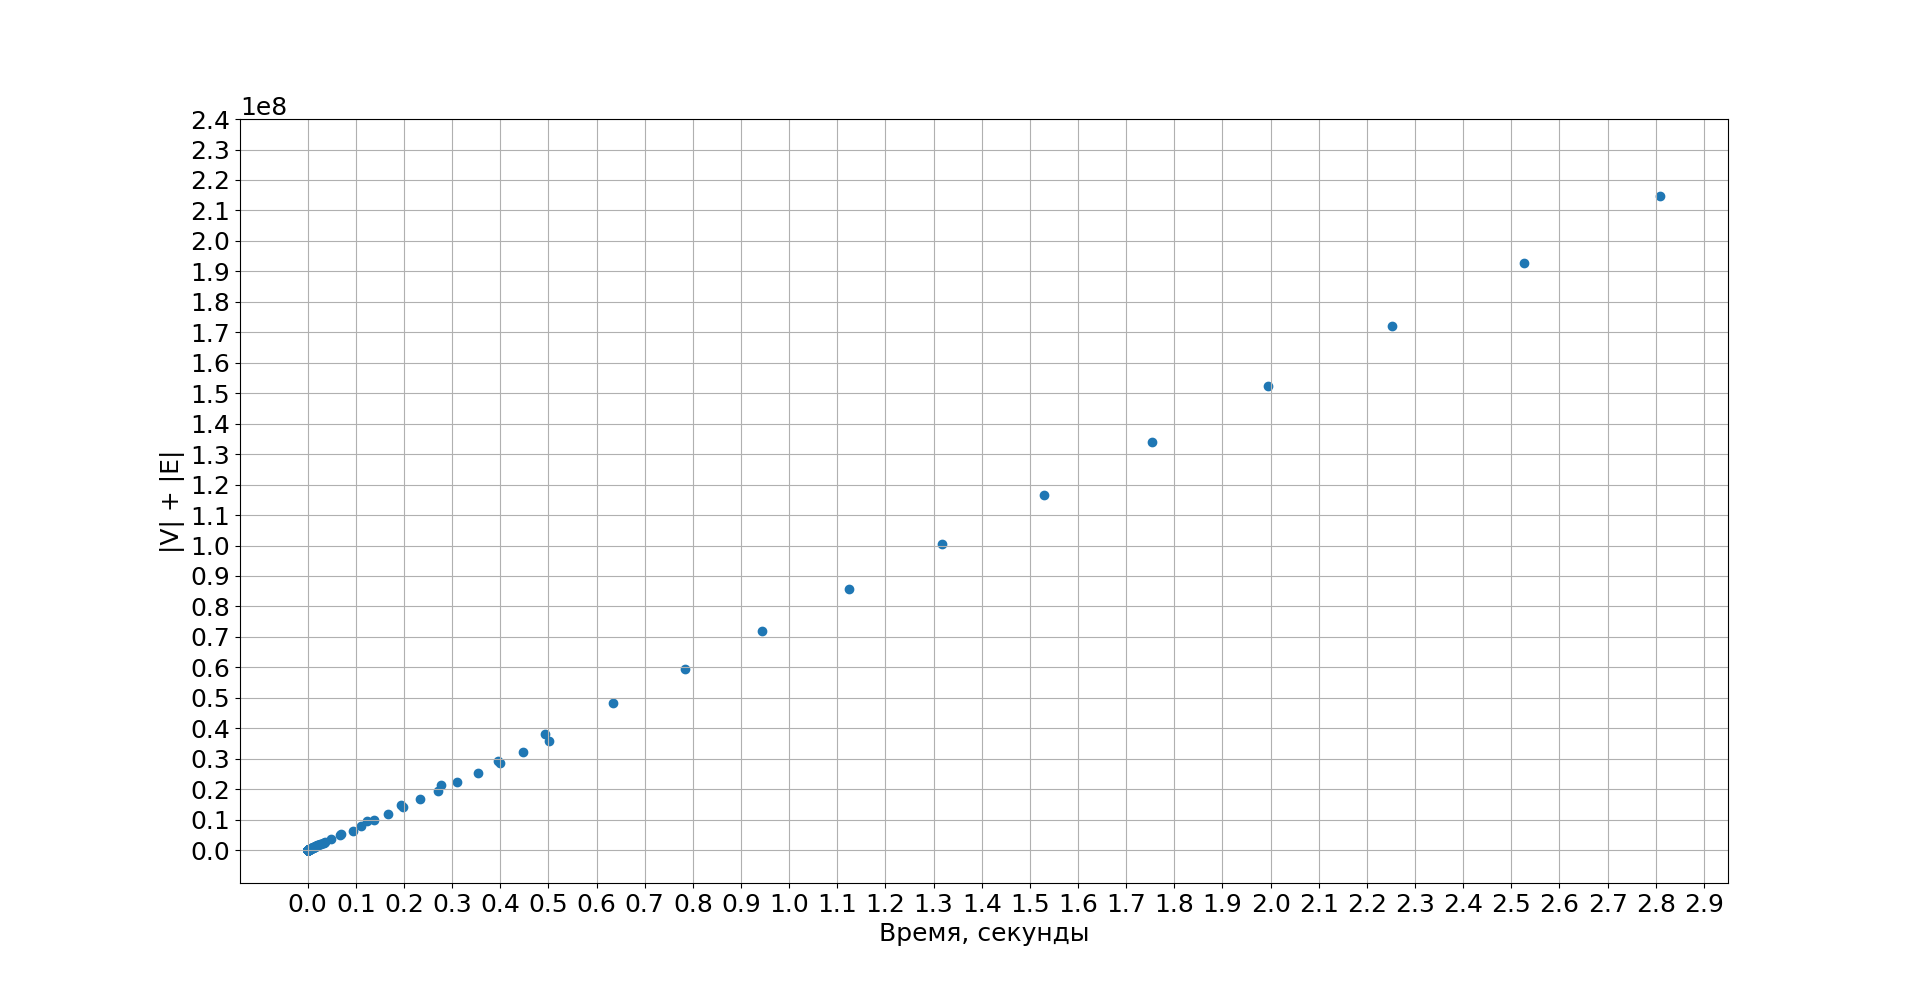
\includegraphics[width=1\linewidth]{figure_1}}
    \caption{Зависимость времени выполнения алгоритма от суммы количества 
    вершин и количества рёбер}
\end{figure}

\newpage
\section{Анализ результатов.}
\noindent
Полученные результаты запуска алгоритма доказывают правильность априорного
исследования влияния входных данных на время выполнения алгоритма.\\
Алгоритм
Тарьяна поиска компонент сильной связности графа рабоает за линейное время
относительно входных данных (количество вершин и рёбер).\\

\newpage
\section{Список литературы.}
\noindent
1) https://github.com/egorka001/Algorithms\_and\_Complexity/tree/main - 
репозиторий с кодом проекта\\
2) Tarjan R. E. Depth-first search and linear graph algorithms (англ.) // 
SIAM Journal on Computing. — 1972.\\ 
3) Donald Knuthi, The Stanford GraphBase \\
4) Е. Просолупов, Курс лекций по дискретной математике. Часть 3. 
Теория алгоритмов и теория графов\\

\newpage
\section{Оборудование.}
\noindent
1) Компилятор: gcc, version: 11.3.0\\
2) Процессор: Intel Core i5-5200U @ 4x 2.7GHz\\
3) RAM: 11872MiB\\
4) OS: Ubuntu 22.04 jammy\\
5) Kernel: x86\_64 Linux 5.15.0-53-generic

\end{document}
